\documentclass[dvipsnames,parskip,a4paper]{scrartcl}

% Color and design packages
\usepackage[usenames,dvipsnames]{xcolor}
\usepackage{tikz}
\usetikzlibrary{positioning}

\usepackage{pifont}
\usepackage{graphicx}
\usepackage{etoolbox}
\usepackage{longtable}
\usepackage{fontspec}
\usepackage[export]{adjustbox}
\usepackage[utf8]{inputenc}
\usepackage[margin=1.5cm]{geometry}
\usepackage{nopageno}
\usepackage{titling}

\setlength{\parskip}{0pt}
\setlength{\tabcolsep}{0pt}

% Clear date
\predate{}
\postdate{}
\date{}

\title{Elemental Dice}
\author{Emil Indzhev}

% Card sizing
\newcommand{\cardroundingradius}{4mm}
\newcommand{\cardboxroundingradius}{0.5mm}
\newcommand{\cardtextborderspace}{1.28mm}
\newcommand{\cardwidth}{57.5mm}
\newcommand{\cardheight}{89mm}
\newcommand{\cardtitleheight}{7.1mm}
\newcommand{\cardtextheight}{15.8mm}
\newcommand{\cardtcheight}{6mm}
\newcommand{\cardborderspace}{3mm}
\newcommand{\cardvspace}{2.5mm}

\newcommand{\iconsize}{3.4mm}
\newcommand{\icondepth}{0.45mm}

\newcommand{\cardimgborderspace}{0.1mm}
\newcommand{\cardimgwidth}{51.3mm}
\newcommand{\cardimgheight}{46.4mm}
\newcommand{\cardimghalfwidth}{25.65mm}
\newcommand{\cardimghalfheight}{23.2mm}

% Consistent colors
\newcommand{\cardcolormod}{!100}
\newcommand{\cardboxcolormod}{!50}
\newcommand{\cardboxbordercolormod}{!75!black}
\newcommand{\cardbordercolormod}{!75!black}

% Card template
\newcommand{\card}[6]{

\begin{tikzpicture}[baseline = (current bounding box.center)]
\draw[rounded corners = \cardroundingradius, fill = #3\cardcolormod, draw = #3\cardbordercolormod, thick] (0,0) rectangle
    (\cardwidth, \cardheight);

\node (title) at (0.5 * \cardwidth, \cardheight - \cardborderspace)
    [ anchor = north, fill = #3\cardboxcolormod, draw = #3\cardboxbordercolormod, thick, text centered, 
    rounded corners = \cardboxroundingradius,
    inner sep = \cardtextborderspace,
    text width = \cardwidth - 2 * (\cardborderspace + \cardtextborderspace),
    minimum height = \cardtitleheight]
    { \Large #1 };

\node (image) at (0.5 * \cardwidth, \cardborderspace + \cardtcheight + \cardtextheight + 2 * \cardvspace)
    [ anchor = south, fill = #3\cardboxcolormod, thick, text centered,
    rounded corners = \cardboxroundingradius,
    inner sep = \cardimgborderspace,
    text width = \cardwidth - 2 * (\cardborderspace + \cardimgborderspace),
    minimum height = \cardheight - \cardtcheight - \cardtextheight - \cardtitleheight - 2 * \cardborderspace - 3 * \cardvspace]
    {\includegraphics[max size={\cardimgwidth}{\cardimgheight}, min size={\cardimgwidth}{\cardimgheight}, Clip*={.5\width-\cardimghalfwidth} {.5\height-\cardimghalfheight} {.5\width+\cardimghalfwidth} {.5\height+\cardimghalfheight}]{ #6 }};

\node (image_border) at (0.5 * \cardwidth, \cardborderspace + \cardtcheight + \cardtextheight + 2 * \cardvspace)
    [ anchor = south, draw = #3\cardboxbordercolormod, thick, text centered,
    rounded corners = \cardboxroundingradius,
    inner sep = \cardimgborderspace,
    text width = \cardwidth - 2 * (\cardborderspace + \cardimgborderspace),
    minimum height = \cardheight - \cardtcheight - \cardtextheight - \cardtitleheight - 2 * \cardborderspace - 3 * \cardvspace]
    {};

\node (text) at (0.5 * \cardwidth, \cardborderspace + \cardtcheight + \cardvspace)
    [ anchor = south, fill = #3\cardboxcolormod, draw = #3\cardboxbordercolormod, thick, text centered,
    rounded corners = \cardboxroundingradius,
    inner sep = \cardtextborderspace,
    text width = \cardwidth - 2 * (\cardborderspace + \cardtextborderspace),
    minimum height = \cardtextheight]
    { #4 };

\node (type)
    [ fill = #3\cardboxcolormod, draw = #3\cardboxbordercolormod, thick,
    below left = \cardvspace + \cardtcheight and 0mm of text, anchor = south west,
    rounded corners = \cardboxroundingradius,
    inner sep = \cardtextborderspace,
    minimum height = \cardtcheight]
    { #2 };

\node (cost)
    [ fill = #3\cardboxcolormod, draw = #3\cardboxbordercolormod, thick,
    below right = \cardvspace + \cardtcheight and 0mm of text, anchor = south east,
    rounded corners = \cardboxroundingradius,
    inner sep = \cardtextborderspace,
    minimum height = \cardtcheight]
    { #5 };

\end{tikzpicture}%

}

% Card type colors
\definecolor{spellcolor}{rgb}{0.73, 0.63, 0.73}
\definecolor{blessingcolor}{rgb}{0.79, 0.77, 0.55}
\definecolor{reliccolor}{rgb}{0.62, 0.67, 0.74}
\definecolor{miraclecolor}{rgb}{0.79, 0.67, 0.55}
\definecolor{cursecolor}{rgb}{0.58, 0.58, 0.58}
\definecolor{neutralcolor}{rgb}{0.7, 0.7, 0.7}
\definecolor{startspellcolor}{rgb}{0.72, 0.67, 0.72}
\definecolor{startblessingcolor}{rgb}{0.74, 0.73, 0.62}

% Elemental symbols
\newcommand{\icon}[1]{\raisebox{-\icondepth}{\includegraphics[height=\iconsize]{ #1 }}}
\newcommand{\chance}{\icon{icons/chance.png}}
\newcommand{\fire}{\icon{icons/fire.png}}
\newcommand{\earth}{\icon{icons/earth.png}}
\newcommand{\water}{\icon{icons/water.png}}
\newcommand{\nature}{\icon{icons/nature.png}}
\newcommand{\magic}{\icon{icons/magic.png}}
\newcommand{\gold}{\icon{icons/gold.png}}

% Costs
\newcommand{\starter}{Starter}
\newcommand{\draft}{Draft}
\newcommand{\onecost}{3 gold}
\newcommand{\twocost}{6 gold}
\newcommand{\threecost}{10 gold}
\newcommand{\fourcost}{15 gold}
\newcommand{\fivecost}{21 gold}

\newcommand{\facedowncost}{2}
\newcommand{\refreshcost}{2}
\newcommand{\refreshcostincrease}{1}
\newcommand{\expresscost}{3}

\newcommand{\startgold}{5}

% Counts and sizes
\newcommand{\handsize}{4}
\newcommand{\facedownsize}{2}
\newcommand{\shopsize}{5}

% HPs
\newcommand{\starthp}{90}
\newcommand{\maxhp}{160}

\begin{document}

\maketitle

\newpage

\subsection*{Summary}

The game is played between two players who build their decks and take turns playing cards from them. Their decks start weak, but they can improve them by buying better cards or removing weak ones. Each player also has some mana (used to play cards), gold (used to buy cards) and HP (if it reaches 0, the player loses). Some cards give gold, deal damage or restore HP, while others provide various forms of utility, shielding or buffs. Seven elemental dice determine the strengths of various cards: Chance \chance, Fire \fire, Earth \earth, Water \water, Nature \nature, Gold \gold \ and Magic \magic. They are rolled at the start and stay like that. However, some cards can change the values of these dice, thus changing how strong other cards are.

\subsection*{Win condition}

The game ends in one of two cases:

\begin{itemize}
\item A player's HP reaches 0 (or less). Then the other player wins. If both players' HPs reach 0 at the same time, the winner is the player whose card dealt the final damage.
\item A player's HP reaches \maxhp \ (or more). Then they win. (Cannot happen to both players simultaneously.)
\end{itemize}

\subsection*{The cards}

There are some \starter \ and \draft \ cards, which each player's deck starts with. The rest are buyable from the shop and have gold costs: \onecost, \twocost, \threecost, \fourcost \ or \fivecost.

\vspace{4pt}

Mechanically, there are 5 types of cards (listed in order of decreasing commonness):

\begin{itemize}
\item Spells -- Go into a player's deck upon being bought and cost 1 mana to play.
\item Blessings -- Similar to spells, but cost no mana and can also be played during the opponent's turn.
\item Relics -- Deployed immediately upon being bought and remain in play until the end of the game.
\item Miracles -- Only have effects upon being bought and then they trash themselves.
\item Curses -- Go into the opponent's deck upon being bought and are unplayable.
\end{itemize}

Playable cards (spells and blessings) can also be placed face down at a cost of 1 mana and 2 gold and then be flipped later like a blessing: at no cost and potentially during the opponent's turn.

\vspace{4pt}

We can also classify most cards depending on what they do:

\begin{itemize}
\item Attack -- ``Deal X damage'' cards (i.e. reduce the opponent's HP). They scale with one or two of \chance, \fire, \earth, \water \ and \magic. Attacks that scale with \water \ deal damage to both players.
\item Restore -- ``Restore X HP'' cards. They scale with \nature \ and possibly one of the attack elements.
\item Gold -- ``Gain X gold'' cards. They scale with \gold \ and possibly one of the attack elements.
\item Buff -- ``Double the strength of all your cards scaling with X'' cards. They buff other cards.
\item Shield -- ``Shield X against damage scaling with Y'' cards. They reduce incoming damage.
\item Dice Control -- various cards that affect the dice (either changing their values or rerolling them). These are the only way to change the dice values (and thus affect how strong various other cards are).
\item Draw -- ``Draw X cards'' cards. Useful for finding the valuable cards.
\item Mana -- ``Gain X mana'' cards. Useful for playing multiple spells in a single turn.
\item Trash -- ``Trash X cards from ...'' cards. Trashing a card means moving it to the trash pile, making it permanently inaccessible by anything. Useful for removing weak cards.
\item Other utility -- various other cards with hard to categorize effects. Some may allow seeing otherwise hidden information or messing with the opponent in some way, etc.
\end{itemize}

\subsection*{Elemental scaling}

Many cards' descriptions have an element symbol instead of a number, e.g. ``Deal \fire \ damage to your opponent''. This means that the amount of damage dealt is equal to the current value of the \fire \ die. We say that this card scales with \fire. Note that the die is not rerolled when playing such a card.

\vspace{4pt}

It is also possible to have a stronger scaling like 2\hspace{1pt}$\times$\hspace{1pt}\fire, which would mean that the damage is equal to 2 times the current value of the \fire \ die. Other cards may scale with multiple elements like \earth\hspace{1pt}$+$\hspace{1pt}\chance \ or \water\hspace{1pt}\times\hspace{1pt}\magic, which would mean that the damage is equal to sum or product, respectively, of the current values of the two listed dice.

\vspace{4pt}

In all multi-element scaling cards, the combination is a sum, if neither element is \magic, and a product, otherwise. There are no single-element \magic \ scaling cards, i.e. \magic \ is always a multiplier for another element.

\vspace{4pt}

\subsection*{The \chance \ die}

Unlike all other dice, whenever its value is needed by a card that scales with it, it is rerolled before executing (and calculating the strength of) the card. Note that dice control cards can still affect the \chance \ die, though this usually achieves nothing.

\subsection*{Buffs}

Buffs (``Double the strength of all your cards scaling with X until the end of your turn.'') work by doubling the effective values of all dice except \magic \ in the strength calculations for all cards (of the player with the buff) that scale with X (and possibly something else). Multiple buffs can affect the same cards (i.e. two buffs means times 4). Buffs are discarded at the end of the player's turn (i.e. if played during the opponent's turn, a buff lasts through that and the player's turn.)

\vspace{4pt}

Example: Alice plays buff that targets \fire. She then plays a \fire\hspace{1pt}$\times$\hspace{1pt}\magic \ attack, a \nature\hspace{1pt}$+$\hspace{1pt}\fire \ restore and a \water\hspace{1pt}$+$\hspace{1pt}\earth \ attack. The first two will be doubled (i.e. will do 2\hspace{1pt}$\times$\hspace{1pt}\fire\hspace{1pt}$\times$\hspace{1pt}\magic \ damage and 2\hspace{1pt}$\times$\hspace{1pt}\nature\hspace{1pt}$+$\hspace{1pt}2\hspace{1pt}$\times$\hspace{1pt}\fire \ restoration, respectively), while the last attack will not be doubled.

\subsection*{Shields}

Shields (``Shield X against damage scaling with Y until the end of your opponent's turn'') work by subtracting (without going negative) the value of die X from all dice except \magic \ in the strength calculations for all incoming damage (towards the player with the shield) that scales with X (and possibly something else). Multiple shields can affect the same card. Shields are discarded at the end of the opponent's turn (i.e. if played during the player's turn, a shield lasts through that and the opponent's turn.)

\vspace{4pt}

This shield subtraction happens after the doubling due to buffs. Both the shield and/or the incoming damage can be buffed. In the first case, the substracted value is doubled. In the second case, the value(s) being subtracted from is/are doubled.

\vspace{4pt}

Example: During her turn, Alice plays a \fire \ buff and a 2\hspace{1pt}$\times$\hspace{1pt}\fire \ attack. The value of the \fire \ die is 4, so this attack would deal $2 \times 2 \times 4 = 16$ damage. However, Bob counters by playing a \water \ shield against \fire. The value of the \water \ die is 3, so the attack now deals $2 \times (2 \times 4 - 3) = 10$ damage. Had Bob also played a \water \ buff, the attack would have dealt $2 \times (2 \times 4 - 2 \times 3) = 4$.

\vspace{4pt}

Example 2: Alice plays a \water\hspace{1pt}$+$\hspace{1pt}\earth \ attack that targets both players. The value of the \water \ die is 2 and that of the \earth \ one is 5, so this attack would deal $2 + 5 = 7$ damage to both players. However, Alice has already played a \magic \ shield against multi-element damage. The value of the \magic \ die is 4. The attack now deals $0 + (5 - 4) = 1$ damage to Alice (since $2 - 4$ is negative) and still 5 damage to Bob.

\subsection*{Gold}

Gold (represented by the coins) is gained passively (1 per turn) and by playing cards. Other than with gold cards: A player dealing damage or restoring HP (to their opponent or themselves) receives gold equal to half the damage dealt/HP restored (rounded up). Note that, if a card deals damage to both players, the gold gained is half of the total damage dealt. Gold is mainly spent on refreshing the shop, buying cards or placing face down cards.

\subsection*{Initial setup}

\begin{itemize}
\item Each player starts with \starthp \ HP (out of \maxhp) and \startgold \ gold.
\item All seven elemental dice are rolled and ordered next to the HP tracker like so: \chance, \fire, \earth, \water, \nature, \gold, \magic.
\item All cards with gold costs are shuffled together and form the shop's draw pile. No shop cards are laid out at the start.
\item The 8 \draft \ cards (``Fire'', ``Tremor'', ``Heavy Rain'', ``Blind Attack'', ``Flower Gardens'', ``Marketplace'', ``Gambling'' and ``Cheap Trick'') are shuffled together; 6 of them are dealt out and the other 2 are trashed.
\item Each player rolls a die and whoever rolls higher chooses who goes first. (In case of a tie, reroll.)
\item The player who rolled lower in the first player determination can decide to swap who goes first and who goes second by offering 1 advantage (ability to change a die by 1) to the other player. If this happens, the other player has the same option, but for 2 advantage. This repeats (with increasing advantage numbers) until one player passes up on using this option. Only the final advantage offer remains in effect, as this is effectively an auction for the turn order.
\item The first player drafts (chooses) 1 of the dealt out \draft \ cards, the second one drafts 2 of the remaining ones, the first one drafts 2, and the last card goes to the second player.
\item The starting draw pile of each player is formed by shuffling together the 9 Starter cards (8 ``Basic Income'' and 1 ``Lucky Find'') and their 3 chosen \draft \ cards.
\item The player with X advantage (if any) can change the value of a die by 1 up to X times (can be the same die, different dice or any other combination).
\item Each player draws \handsize \ cards from their draw pile into their hand and the first player starts their turn.
\end{itemize}

\subsection*{A player's turn}

At the start of their turn, the player gains 1 gold and 1 mana. After that they can do any of the following actions (in any order, possibly multiple times and/or interleaved):

\begin{itemize}
\item Play a spell from their hand at the cost of 1 mana.
\item Play a blessing from their hand at no cost.
\item Place a playable card (spell or blessing) from their hand face down at the cost of 1 mana and \facedowncost \ gold. A player can have at most \facedownsize \ face down cards at a time.
\item Play (flip over and activate) a face down card at no cost.
\item Refresh the shop. The first refresh in a given turn costs \refreshcost \ gold and each subsequent is \refreshcostincrease \ gold more expensive.
Refreshing the shop consists of moving the currently laid out shop cards (if any) to the shop's discard pile followed by drawing and laying out \shopsize \ cards from the shop's draw pile. Note that initially there are no shop cards laid out.
\item Buy a card from the laid out shop cards by paying its cost.
The bought card is not replaced, so the shop can become empty again. If the card is a playable card (spell or blessing), it goes into the player's discard pile; if it is a relic, it is immediately and permanently deployed; if it is a miracle, it is immediately trashed; if it is a curse, it goes goes into the opponent's discard pile.
\end{itemize}

Whenever a card is played, it is initially active. Once its effect is executed/expires (instantly for most cards), it becomes inactive and is set to the side to be discarded at the end of the turn. Active cards are kept in the main play area and may persist between turns.

\vspace{4pt}

After the current player declares their turn to be over, they lose all their mana and discard their entire hand, both players discard their inactive played cards and then the current player draws \handsize \ cards from their draw pile. Finally, the opponent's turn starts, but before they can act, the current player can play any number of off-turn cards (blessings or face down cards) until they declare that they are done.

\subsection*{Interruptions from the opponent}

Whenever a player plays a spell that scales with an element/elements (i.e. an attack, a restore or a gold card), their opponent (regardless of whose turn it is) can interrupt it before it is executed (rolling the \chance \ die due to its rule is considered part of the execution). The interrupted card is rotated by 90 degrees clockwise to indicate that it is yet to be executed. Then the opponent can do any number of actions valid for them. After they declare that they are done the interrupted player has the chance to do the same. This can repeat any number of times (i.e. the opponent going again, then the interrupted player, etc.) until one of the players chooses to do nothing (i.e. declares being done without doing any actions). After that the interrupted card is executed (and its rotation is undone). Then the turn continues as it would have, had the interruption not happened, i.e. the initiative returns to the player whose card was interrupted.

\vspace{4pt}

Note that both players can only do actions valid for them. This is restricted to only playing off-turn cards (blessings and face down cards) for the player whose turn it is not (regardless of whether they are interrupting or being interrupted). However, for the player whose turn it is, all the usual actions are valid, including: playing spells from their hand, placing face down cards and even interacting with the shop.

\vspace{4pt}

Also note that, in case there are multiple interrupted cards at the same time, it is important to keep track of their order (as they would be resolved from last to first, with a chance to continue doing actions between each), so lay them out in a time line.

\vspace{4pt}

Example: In a very close game, Alice is at 4 HP and Bob at 2 HP. During her turn, Alice plays a \fire \ attack. The current value of \fire \ is 6, so she would win. Bob interrupts this and flips a face down card that allows him to reroll the \fire \ die. It rolls a 2, so he is still losing. Then, he plays a blessing from his hand: a \water \ shield against \fire \ attacks. The value of \water \ is 4, so this would mitigate all damage. He is done for now. Alice then plays a blessing that gives her mana, allowing her to play another spell (from her hand): ``Trickster God'', which she uses to swap the values of the \fire \ and \water \ dice. Bob is again losing so he flips his second face down card: a \chance \ attack, which has a 50\% chance of winning him the game. Alice interrupts this by playing a \gold \ shield against single element attacks. The value of \gold \ is 2, so Bob needs a 6 to win. Alice is done and Bob passes as he has nothing more to do. He rolls the \chace \ die to execute his attack, but the die lands on a 4. He is done. Alice is also done. Finally, Alice's attack is executed and she wins the game.

\subsection*{Discard pile}

Whenever a player needs to discard some number of cards (from their hand or face down cards), but has fewer than that, they simply discard all such cards and that effect is considered as executed. Instead, if the player has more cards than that, they chose which cards to discard.

\vspace*{4pt}

Whenever a card needs to be drawn from a deck's draw pile, but it is empty, its discard pile is shuffled and it becomes the draw pile. This is never triggered by effects without the ``draw'' keyword (e.g. ``Look at top X cards of your draw pile'', even if the draw pile has fewer than X cards).

\subsection*{Private and public information}

A player's hand, face down cards, discard pile and discards are private information, i.e. only they can see them. The laid out shop, the shop's discard pile, the trash pile, a player's played cards, bought cards, trashed cards, gold, HP, mana and all counts (e.g. number of cards in hand) are all public information, i.e. everyone can see them. All draw piles are hidden information, i.e. nobody can see them.

\subsection*{Trackers and tokens}

Use the 7 colored dice for the elements. Use the spare dice to roll for turn order choice. Use the HP tracker (the large grid) and the two differently colored pawns to keep track of players' HPs. Use the coins to keep track of players' gold. If needed, use the spare dice or other tokens to keep track of mana.

\subsection*{Resigning}

If at any point, a player no longer wishes to continue, they can resign. This means they lose the game and their opponent wins. This is a full-fledged victory. However, resigning too easily or right before one's opponent is about to pull off a big combo is discouraged.

\subsection*{Card Clarifications}

\begin{itemize}
\item ``Second Chance'', ``Sleight of Hand'', ``Calculated Risk'' and ``Smoke and Mirrors'' affect only one die (chosen by the player), i.e. their effects cannot be split up over multiple dice.
\item ``Wish'' and ``Scout'' can target cards in the shop and its draw and discard piles, but not trashed cards.
\item ``At What Cost'', when bought, must trash itself, if the player owns no other relics.
\item ``Vicious Curse'' does not prevent the trashing of relics, only of cards in the player's deck.
\item ``Veto'' is active until the start of the opponent's next turn.
\end{itemize}

\newpage

\begin{longtable}{ c c c }

\card{Fire}{Spell}{spellcolor}{Deal \fire \ damage to your opponent.}{\draft}{imgs/fire.png}
&
\card{Tremor}{Spell}{spellcolor}{Deal \earth \ damage to your opponent.}{\draft}{imgs/tremor.png}
&
\card{Heavy Rain}{Spell}{spellcolor}{ \small Deal \water \ damage to your opponent and yourself; opponent shields affect self damage.}{\draft}{imgs/heavy_rain.png}
&
\card{Blind Attack}{Spell}{spellcolor}{Deal \chance \ damage to your opponent.}{\draft}{imgs/blind_attack.png}
&
\card{Blazing Fire}{Spell}{spellcolor}{Deal 2\hspace{1pt}$\times$\hspace{1pt}\fire \ damage to your opponent.}{\threecost}{imgs/blazing_fire.png}
&
\card{Massive Earthquake}{Spell}{spellcolor}{Deal 2\hspace{1pt}$\times$\hspace{1pt}\earth \ damage to your opponent.}{\threecost}{imgs/massive_earthquake.png}
&
\card{Torrential Rainstorm}{Spell}{spellcolor}{ \small Deal 2\hspace{1pt}$\times$\hspace{1pt}\water \ damage to your opponent and yourself; opponent shields affect self damage.}{\threecost}{imgs/torrential_rainstorm.png}
&
\card{Haphazard Offence}{Spell}{spellcolor}{Deal 2\hspace{1pt}$\times$\hspace{1pt}\chance \ to your opponent.}{\threecost}{imgs/haphazard_offence.png}
&
\card{Lava Surge}{Spell}{spellcolor}{Deal \fire\hspace{1pt}$+$\hspace{1pt}\earth \ damage to your opponent.}{\threecost}{imgs/lava_surge.png}
&
\card{Erratic Blaze}{Spell}{spellcolor}{Deal \fire\hspace{1pt}$+$\hspace{1pt}\chance \ damage to your opponent.}{\threecost}{imgs/erratic_blaze.png}
&
\card{Chaotic Avalanche}{Spell}{spellcolor}{Deal \earth\hspace{1pt}$+$\hspace{1pt}\chance \ damage to your opponent.}{\threecost}{imgs/chaotic_avalanche.png}
&
\card{Scalding Fog}{Spell}{spellcolor}{ \small Deal \water\hspace{1pt}$+$\hspace{1pt}\fire \ damage to your opponent and yourself; opponent shields affect self damage.}{\threecost}{imgs/scalding_fog.png}
&
\card{Devastating Mudslide}{Spell}{spellcolor}{ \small Deal \water\hspace{1pt}$+$\hspace{1pt}\earth \ damage to your opponent and yourself; opponent shields affect self damage.}{\threecost}{imgs/devastating_mudslide.png}
&
\card{Wild Seas}{Spell}{spellcolor}{ \small Deal \water\hspace{1pt}$+$\hspace{1pt}\chance \ damage to your opponent and yourself; opponent shields affect self damage.}{\threecost}{imgs/wild_seas.png}
&
\card{Magical Inferno}{Spell}{spellcolor}{Deal \fire\hspace{1pt}$\times$\hspace{1pt}\magic \ damage to your opponent.}{\fourcost}{imgs/magical_inferno.png}
&
\card{Arcane Meteor}{Spell}{spellcolor}{Deal \earth\hspace{1pt}$\times$\hspace{1pt}\magic \ damage to your opponent.}{\fourcost}{imgs/arcane_meteor.png}
&
\card{Biblical Flood}{Spell}{spellcolor}{ \small Deal \water\hspace{1pt}$\times$\hspace{1pt}\magic \ damage to your opponent and yourself; opponent shields affect self damage.}{\fourcost}{imgs/biblical_flood.png}
&
\card{Ethereal Havoc}{Spell}{spellcolor}{Deal \chance\hspace{1pt}$\times$\hspace{1pt}\magic \ damage to your opponent.}{\fourcost}{imgs/ethereal_havoc.png}
&

\card{Flower Gardens}{Spell}{spellcolor}{Restore \nature \ HP.}{\draft}{imgs/flower_gardens.png}
&
\card{Lush Forests}{Spell}{spellcolor}{Restore 2\hspace{1pt}$\times$\hspace{1pt}\nature \ HP.}{\threecost}{imgs/lush_forests.png}
&
\card{Controlled Burn}{Spell}{spellcolor}{Restore \nature\hspace{1pt}$+$\hspace{1pt}\fire \ HP.}{\threecost}{imgs/controlled_burn.png}
&
\card{Fertile Soils}{Spell}{spellcolor}{Restore \nature\hspace{1pt}$+$\hspace{1pt}\earth \ HP.}{\threecost}{imgs/fertile_soils.png}
&
\card{Hot Springs}{Spell}{spellcolor}{Restore \nature\hspace{1pt}$+$\hspace{1pt}\water \ HP.}{\threecost}{imgs/hot_springs.png}
& 
\card{Clover Fields}{Spell}{spellcolor}{Restore \nature\hspace{1pt}$+$\hspace{1pt}\chance \ HP.}{\threecost}{imgs/clover_fields.png}
&
\card{Mystical Restoration}{Spell}{spellcolor}{Restore \nature\hspace{1pt}$\times$\hspace{1pt}\magic \ HP.}{\fourcost}{imgs/mystical_restoration.png}
&

\card{Marketplace}{Spell}{spellcolor}{Gain \gold \ gold.}{\draft}{imgs/marketplace.png}
&
\card{Treasury}{Spell}{spellcolor}{Gain 2\hspace{1pt}$\times$\hspace{1pt}\gold \ gold.}{\threecost}{imgs/treasury.png}
&
\card{Gold Foundry}{Spell}{spellcolor}{Gain \gold\hspace{1pt}$+$\hspace{1pt}\fire \ gold.}{\threecost}{imgs/gold_foundry.png}
&
\card{Gold Mine}{Spell}{spellcolor}{Gain \gold\hspace{1pt}$+$\hspace{1pt}\earth \ gold.}{\threecost}{imgs/gold_mine.png}
&
\card{Gold Panning}{Spell}{spellcolor}{Gain \gold\hspace{1pt}$+$\hspace{1pt}\water \ gold.}{\threecost}{imgs/gold_panning.png}
&
\card{Free Market}{Spell}{spellcolor}{Gain \gold\hspace{1pt}$+$\hspace{1pt}\chance \ gold.}{\threecost}{imgs/free_market.png}
&
\card{Ancient Alchemy}{Spell}{spellcolor}{Gain \gold\hspace{1pt}$\times$\hspace{1pt}\magic \ gold.}{\fourcost}{imgs/ancient_alchemy.png}
&

\card{Water Reservoirs}{Blessing}{blessingcolor}{ \small Shield \water \ against damage scaling with \fire \ until the end of your opponent's turn.}{\onecost}{imgs/water_reservoirs.png}
&
\card{Solid Infrastructure}{Blessing}{blessingcolor}{ \small Shield \earth \ against damage scaling with \water \ until the end of your opponent's turn.}{\onecost}{imgs/solid_infrastructure.png}
&
\card{Natural Forests}{Blessing}{blessingcolor}{ \small Shield \nature \ against damage scaling with \earth \ until the end of your opponent's turn.}{\onecost}{imgs/natural_forests.png}
&
\card{Paid Militia}{Blessing}{blessingcolor}{ \footnotesize Shield \gold \ against damage scaling with a single element until the end of your opponent's turn.}{\twocost}{imgs/paid_militia.png}
&
\card{Magical Barrier}{Blessing}{blessingcolor}{ \footnotesize Shield \magic \ against damage scaling with multiple elements until the end of your opponent's turn.}{\twocost}{imgs/magical_barrier.png}
&

\card{Prometheus's Gift}{Spell}{spellcolor}{Double the strength of all your cards scaling with \fire \ until the end of your turn.}{\twocost}{imgs/prometheuss_gift.png}
&
\card{Gaia's Favor}{Spell}{spellcolor}{Double the strength of all your cards scaling with \earth \ until the end of your turn.}{\twocost}{imgs/gaias_favor.png}
&
\card{Poseidon's Trident}{Spell}{spellcolor}{Double the strength of all your cards scaling with \water \ until the end of your turn.}{\twocost}{imgs/poseidons_trident.png}
&
\card{Ancient Grimoire}{Spell}{spellcolor}{Double the strength of all your cards scaling with \magic \ until the end of your turn.}{\twocost}{imgs/ancient_grimoire.png}
&
\card{Nymphs' Grace}{Spell}{spellcolor}{Double the strength of all your cards scaling with \nature \ until the end of your turn.}{\twocost}{imgs/nymphs_grace.png}
&
\card{Midas Touch}{Spell}{spellcolor}{Double the strength of all your cards scaling with \gold \ until the end of your turn.}{\twocost}{imgs/midas_touch.png}
&
\card{Purism}{Spell}{spellcolor}{ \footnotesize Double the strength of all your cards scaling with a single element until the end of your turn.}{\twocost}{imgs/purism.png}
&

\card{Gambling}{Spell}{spellcolor}{Reroll a die up to 1 time.}{\draft}{imgs/gambling.png}
&
\card{Second Chance}{Spell}{spellcolor}{Reroll a die up to 2 times.}{\twocost}{imgs/second_chance.png}
&
\card{Calculated Risk}{Spell}{spellcolor}{Reroll a die up to 4 times.}{\threecost}{imgs/calculated_risk.png}
&
\card{Cheap Trick}{Spell}{spellcolor}{Change the value of a die by up to 1.}{\draft}{imgs/cheap_trick.png}
&
\card{Sleight of Hand}{Spell}{spellcolor}{Change the value of a die by up to 2.}{\twocost}{imgs/sleight_of_hand.png}
&
\card{Smoke and Mirrors}{Spell}{spellcolor}{Change the value of a die by up to 3.}{\threecost}{imgs/smoke_and_mirrors.png}
&
\card{Perspective Shift}{Spell}{spellcolor}{Flip a die over, i.e. set its value to 7 minus its current value.}{\threecost}{imgs/perspective_shift.png}
&
\card{Trickster God}{Spell}{spellcolor}{Swap the values of a pair of dice.}{\fourcost}{imgs/trickster_god.png}
&
\card{Cosmic Puppeteer}{Spell}{spellcolor}{Change the values of all dice by up to 1 each.}{\fourcost}{imgs/cosmic_puppeteer.png}
&
\card{Madness}{Miracle}{miraclecolor}{Upon buying, reroll all dice.}{\onecost}{imgs/madness.png}
&
\card{Fortuna's Protection}{Relic}{reliccolor}{You choose whether the \chance \ die is rerolled each time its value is needed.}{\threecost}{imgs/fortunas_protection.png}
&

\card{Multitasking Novice}{Blessing}{blessingcolor}{Gain 1 mana.}{\twocost}{imgs/multitasking_novice.png}
&
\card{Multitasking Master}{Blessing}{blessingcolor}{Gain 2 mana.}{\threecost}{imgs/multitasking_master.png}
&
\card{Multitasking Lord}{Blessing}{blessingcolor}{Gain 2 mana and draw a card.}{\fourcost}{imgs/multitasking_lord.png}
&
\card{Multitasking God}{Blessing}{blessingcolor}{Gain 3 mana and draw a card.}{\fivecost}{imgs/multitasking_god.png}
&
\card{Cruel Pact}{Blessing}{blessingcolor}{Take \chance \ damage and gain 1 mana.}{\onecost}{imgs/cruel_pact.png}
&
\card{Deal with the Devil}{Blessing}{blessingcolor}{Take \chance \ damage and gain 2 mana.}{\twocost}{imgs/deal_with_the_devil.png}
&
\card{All for One}{Relic}{reliccolor}{Up to once during your turn, discard 3 cards from your hand and gain 1 mana.}{\twocost}{imgs/all_for_one.png}
&
\card{Clear Mind}{Relic}{reliccolor}{ \small Gain 1 extra mana at the start of your turn, but draw 1 fewer cards after your turn.}{\threecost}{imgs/clear_mind.png}
&
\card{At What Cost}{Relic}{reliccolor}{ \footnotesize Upon buying, trash a relic you own; gain 1 extra mana at the start of your turn.}{\fourcost}{imgs/at_what_cost.png}
&

\card{Exploration Novice}{Spell}{spellcolor}{ \small Draw 2 cards; if this is the first time you play a draw spell during your turn, gain 1 mana.}{\twocost}{imgs/exploration_novice.png}
&
\card{Exploration Master}{Spell}{spellcolor}{ \small Draw 3 cards; if this is the first time you play a draw spell during your turn, gain 1 mana.}{\threecost}{imgs/exploration_master.png}
&
\card{Exploration Lord}{Spell}{spellcolor}{ \small Draw 4 cards; if this is the first time you play a draw spell during your turn, gain 1 mana.}{\fourcost}{imgs/exploration_lord.png}
&
\card{Exploration God}{Spell}{spellcolor}{ \small Draw 5 cards; if this is the first time you play a draw spell during your turn, gain 1 mana.}{\fivecost}{imgs/exploration_god.png}
&
\card{Well-Laid Plans}{Blessing}{blessingcolor}{ \small Reorder the top \handsize \ cards of your draw pile and discard any number of them.}{\twocost}{imgs/well_laid_plans.png}
&
\card{Magnetic Hands}{Blessing}{blessingcolor}{ \small Move any card from your draw pile to your hand and shuffle your draw pile.}{\twocost}{imgs/magnetic_hands.png}
&
\card{Truly Blessed}{Relic}{reliccolor}{ \footnotesize The first time you play a blessing during your turn, draw a card before executing it.}{\threecost}{imgs/truly_blessed.png}
&
\card{Big Handed}{Relic}{reliccolor}{Draw 1 extra card after your turn.}{\fourcost}{imgs/big_handed.png}
&

\card{Optimization Novice}{Spell}{spellcolor}{Trash this card and up to 1 card from your hand.}{\onecost}{imgs/optimization_novice.png}
&
\card{Optimization Master}{Spell}{spellcolor}{Trash this card and up to 2 cards from your hand.}{\twocost}{imgs/optimization_master.png}
&
\card{Optimization Lord}{Spell}{spellcolor}{Trash this card and up to 3 cards from your hand.}{\threecost}{imgs/optimization_lord.png}
&
\card{Optimization God}{Spell}{spellcolor}{Trash this card and up to 3 cards from your hand or discard pile.}{\fourcost}{imgs/optimization_god.png}
&
\card{Spring Cleaning}{Miracle}{miraclecolor}{Upon buying, trash up to 1 card from your hand.}{\twocost}{imgs/spring_cleaning.png}
&

\card{Wish}{Spell}{spellcolor}{ \footnotesize Buy any unowned card for free and shuffle the shop's draw pile; trash this card after 3 uses.}{\fivecost}{imgs/wish.png}
&
\card{Scout}{Miracle}{miraclecolor}{Upon buying, buy any unowned card and shuffle the shop's draw pile.}{\twocost}{imgs/scout.png}
&
\card{Express Shipping}{Relic}{reliccolor}{ \small Whenever you buy a playable card, you can pay \expresscost \ gold for it to go into your hand.}{\twocost}{imgs/express_shipping.png}
&

\card{Mirror Wall}{Blessing}{blessingcolor}{Draw a card and look at your opponent's hand.}{\onecost}{imgs/mirror_wall.png}
&
\card{Mirror Table}{Blessing}{blessingcolor}{Draw a card and look at your opponent's face down cards.}{\onecost}{imgs/mirror_table.png}
&
\card{Sneak Peek}{Blessing}{blessingcolor}{Draw a card and look at the top \handsize \ cards of your draw pile.}{\onecost}{imgs/sneak_peak.png}
&
\card{Forecast}{Blessing}{blessingcolor}{Draw a card and look at the top \shopsize \ cards of the shop's draw pile.}{\onecost}{imgs/forecast.png}
&

\card{Spacious Table}{Relic}{reliccolor}{You have space for 1 extra face down card.}{\twocost}{imgs/spacious_table.png}
&

\card{Merchant's Goodwill}{Relic}{reliccolor}{Your shop refreshes cost 1 less gold.}{\onecost}{imgs/merchants_goodwill.png}
&
\card{Cheapskate}{Relic}{reliccolor}{Face down cards no longer cost you gold to place.}{\twocost}{imgs/cheapskate.png}
&
\card{Trading Vessels}{Relic}{reliccolor}{Gain 1 extra gold at the start of your turn.}{\twocost}{imgs/trading_vessels.png}
&

\card{Veto}{Spell}{spellcolor}{Your opponent receives 1 less mana at the start of their next turn.}{\onecost}{imgs/veto.png}
&
\card{Weak Hands}{Blessing}{blessingcolor}{Your opponent must discard 3 cards from their hand.}{\twocost}{imgs/weak_hands.png}
&
\card{Faulty Table}{Blessing}{blessingcolor}{Your opponent must discard 1 card from their face down cards.}{\twocost}{imgs/faulty_table.png}
&
\card{Sabotage}{Blessing}{blessingcolor}{ \small Reorder the top \handsize \ cards of your opponent's draw pile and discard any number of them.}{\twocost}{imgs/sabotage.png}
&
\card{Curse}{Curse}{cursecolor}{You cannot trash this card.}{\twocost}{imgs/curse.png}
&
\card{Vicious Curse}{Curse}{cursecolor}{You cannot trash any other cards from your deck while this card is in it.}{\threecost}{imgs/vicious_curse.png}
&

\card{Basic Income}{Spell}{startspellcolor}{Gain 1 gold.}{\starter}{imgs/basic_income.png}
&
\card{Basic Income}{Spell}{startspellcolor}{Gain 1 gold.}{\starter}{imgs/basic_income.png}
&
\card{Basic Income}{Spell}{startspellcolor}{Gain 1 gold.}{\starter}{imgs/basic_income.png}
&
\card{Basic Income}{Spell}{startspellcolor}{Gain 1 gold.}{\starter}{imgs/basic_income.png}
&
\card{Basic Income}{Spell}{startspellcolor}{Gain 1 gold.}{\starter}{imgs/basic_income.png}
&
\card{Basic Income}{Spell}{startspellcolor}{Gain 1 gold.}{\starter}{imgs/basic_income.png}
&
\card{Basic Income}{Spell}{startspellcolor}{Gain 1 gold.}{\starter}{imgs/basic_income.png}
&
\card{Basic Income}{Spell}{startspellcolor}{Gain 1 gold.}{\starter}{imgs/basic_income.png}
&
\card{Basic Income}{Spell}{startspellcolor}{Gain 1 gold.}{\starter}{imgs/basic_income.png}
&
\card{Basic Income}{Spell}{startspellcolor}{Gain 1 gold.}{\starter}{imgs/basic_income.png}
&
\card{Basic Income}{Spell}{startspellcolor}{Gain 1 gold.}{\starter}{imgs/basic_income.png}
&
\card{Basic Income}{Spell}{startspellcolor}{Gain 1 gold.}{\starter}{imgs/basic_income.png}
&
\card{Basic Income}{Spell}{startspellcolor}{Gain 1 gold.}{\starter}{imgs/basic_income.png}
&
\card{Basic Income}{Spell}{startspellcolor}{Gain 1 gold.}{\starter}{imgs/basic_income.png}
&
\card{Basic Income}{Spell}{startspellcolor}{Gain 1 gold.}{\starter}{imgs/basic_income.png}
&
\card{Basic Income}{Spell}{startspellcolor}{Gain 1 gold.}{\starter}{imgs/basic_income.png}
&

\card{Lucky Find}{Blessing}{startblessingcolor}{Gain 1 gold.}{\starter}{imgs/lucky_find.png}
&
\card{Lucky Find}{Blessing}{startblessingcolor}{Gain 1 gold.}{\starter}{imgs/lucky_find.png}
&

\card{}{\hspace{30pt}}{neutralcolor}{}{\hspace{30pt}}{}
&
\card{}{\hspace{30pt}}{neutralcolor}{}{\hspace{30pt}}{}
&

\end{longtable}

\newpage

% HP tracker
\begin{tikzpicture}[overlay,remember picture]
\begin{scope}[shift=(current page.center)]
    % Define the grid size
    \def\rows{16}
    \def\cols{10}
    \def\cellsize{16.68mm}
    
    % Calculate the total width and height of the grid
    \def\gridwidth{\cols*\cellsize}
    \def\gridheight{\rows*\cellsize}
    
    % Draw the grid
    \draw[step=\cellsize] (-0.5*\gridwidth, -0.5*\gridheight) grid (0.5*\gridwidth, 0.5*\gridheight);
    
    \foreach \y in {15,...,0}
        \foreach \x in {1,...,10}
            \pgfmathsetmacro\z{int(\x+(10*\y))}
            \node at (-0.5*\gridwidth+\x*\cellsize-\cellsize/2,-0.5*\gridheight+\y*\cellsize+\cellsize/2) {\z};

\end{scope}
\end{tikzpicture}    

\end{document}
